\section{\label{sec:resonances}Comparison of Data to Known States and Cross Sections}

In this section we show a series of figures depicting known resonances with the \abbr{g12} data. The reader is encouraged to compare the masses and widths measured with the PDG\cite{pdg}. The masses of the narrow states in g12 are all measured to be consistent with the known values, such as η in Fig.~\ref{fig:resonances.eta} using the missing mass technique, π$^0$ reconstructed using two photons Fig.~\ref{fig:resonances.2gamma.pi0}, ρ/ω reconstructed using two leptons Fig.~\ref{fig:resonances.ee.rho_omega}, as well as Ξ$^-$ from the reaction of γ π $\rightarrow$ K$^+$ K$^+$ ($X$) shown in Fig.~\ref{fig:resonances.xi}.

\begin{figure}[htpb]\begin{center}
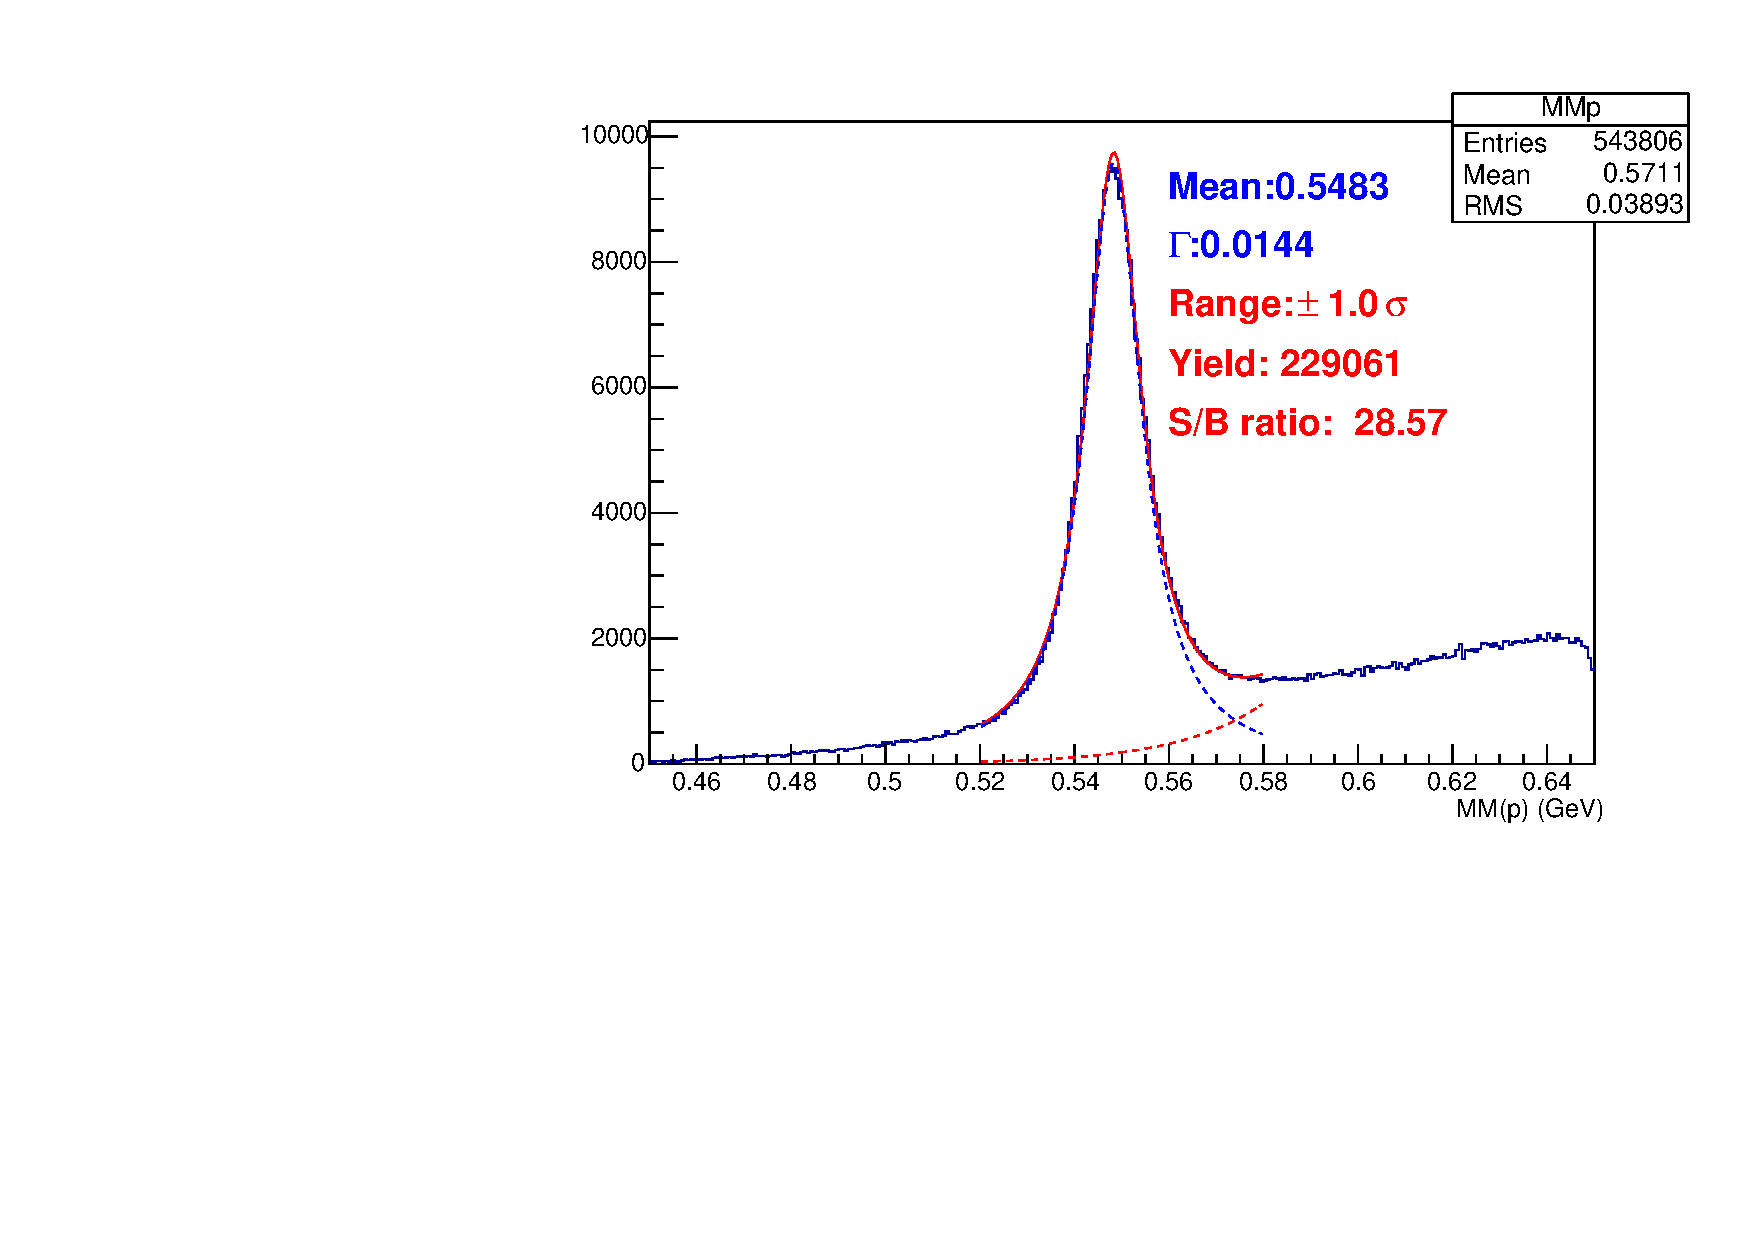
\includegraphics[width=0.4\columnwidth,angle=-90]{{figures/resonances/MMp-eta}.pdf}
\caption[]{\label{fig:resonances.eta}Missing mass off proton showing the η resonance with a measured mass of 548~MeV.}
\end{center}\end{figure}

\begin{figure}[htpb]\begin{center}
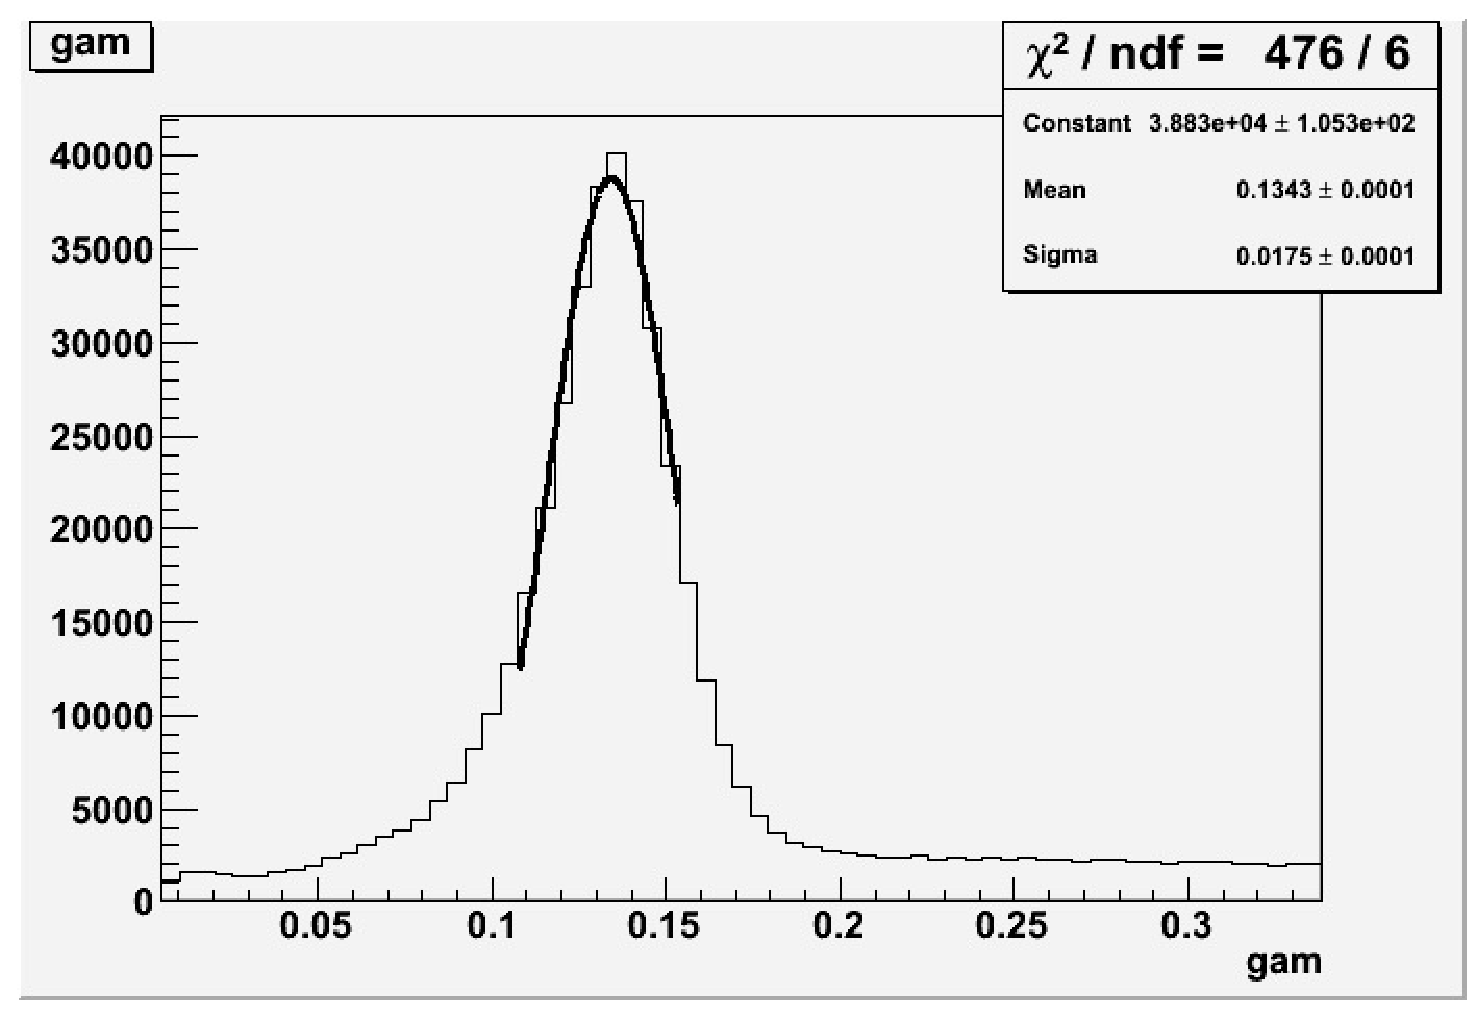
\includegraphics[width=0.4\columnwidth]{{figures/resonances/2gamma-pi0-p2pi2g}.eps}
\caption[]{\label{fig:resonances.2gamma.pi0}Invariant mass of two final-state photons showing the π$^0$ meson.}
\end{center}\end{figure}

\begin{figure}[htpb]\begin{center}
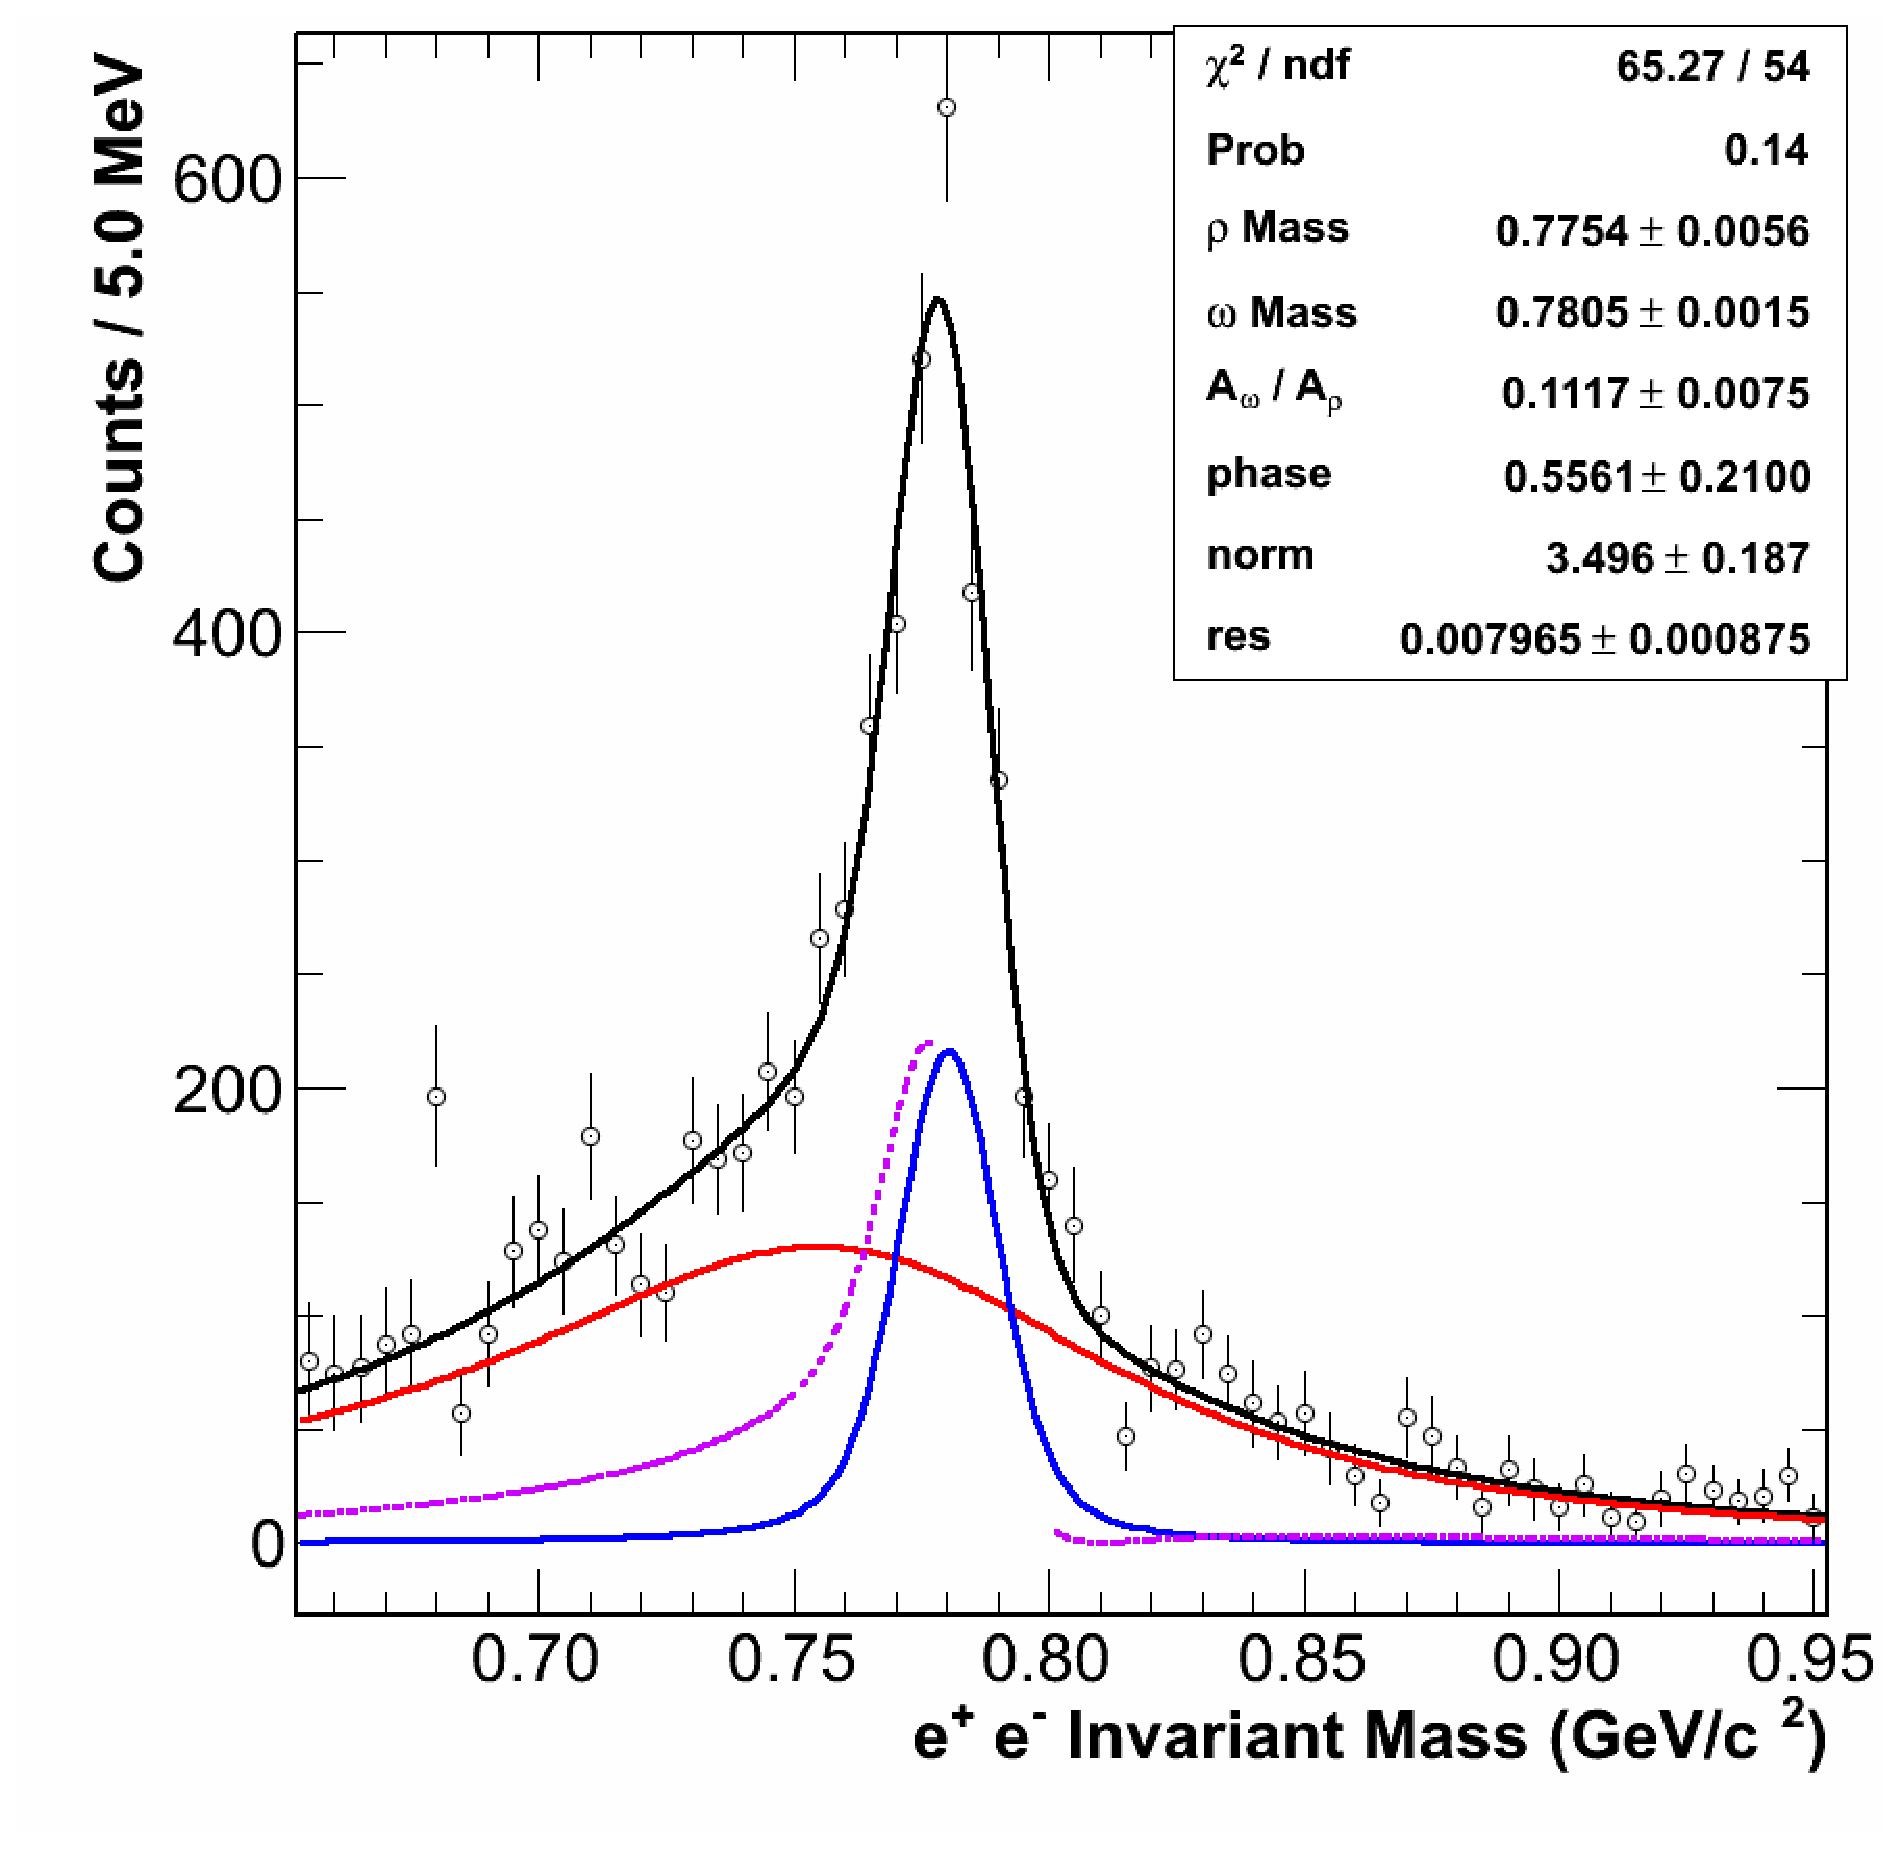
\includegraphics[width=0.4\columnwidth]{{figures/resonances/Sys_NormalRange}.eps}
\caption[]{\label{fig:resonances.ee.rho_omega}Invariant mass of electron and positron pair showing the (mixed) ρ and ω mesons.}
\end{center}\end{figure}


\begin{figure}[htpb]\begin{center}
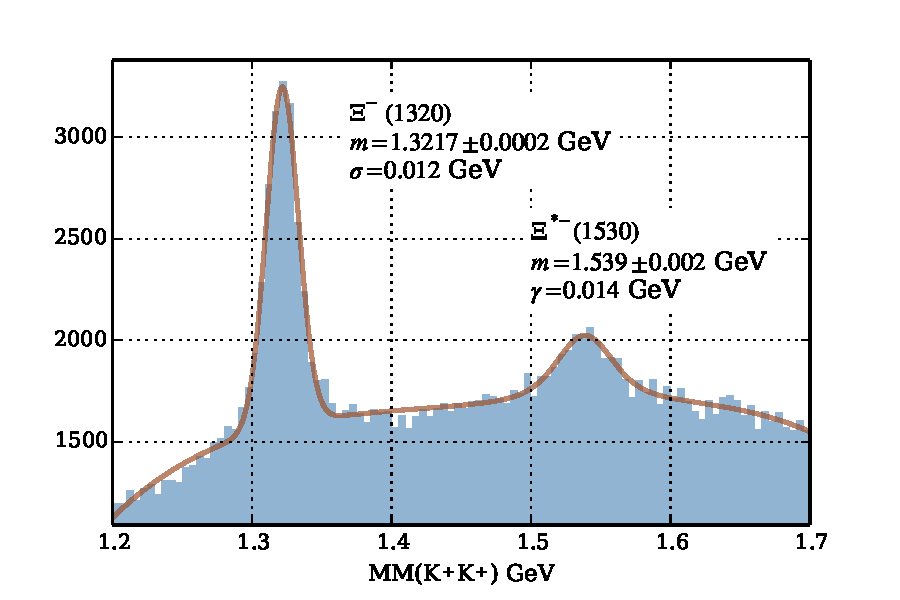
\includegraphics[width=0.4\columnwidth]{{figures/resonances/g12_mmkk_xisignals}.pdf}
\caption[]{\label{fig:resonances.xi}Missing mass off K$^+$K$^+$ showing the ground state and first-excited $\Xi^-$ resonances. The ground state is fit to a Gaussian with a width shown as $σ$, while the first excited state is fit to a Voigtian with a (scaled) Gaussian width taken from the ground state. The value $γ$ shown is the Lorentzian width of the fit.}
\end{center}\end{figure}


\section{\label{sec:xsec}Comparison of Data to Known Cross Sections}

Various cross sections have been extracted using the g12 data set, all showing consistent results when compared with prior CLAS measurements if available, such as the ω, the Λ, as well as π$^0$. In particular, the ω cross section results, measured using γ p $\rightarrow$ p π$^+$ π$^-$ (π$^0$), is presented here and compared with the g11 results and is consistent across the g12 photon energy range. Although some disagreements do show up at particular kinematic bins, it's safe to say that g12 does not have an overall normalization issue.

Figures~\ref{fig:xsec.omega1} and \ref{fig:xsec.omega2} show the differential cross sections for the reaction: γ p $\rightarrow$ p ω, based on the dominant decay mode: ω $\rightarrow$ π$^+$ π$^-$ π$^0$. For this analysis, we have selected events with two positively-charged tracks for the proton and the π$^+$ as well as one negatively-charged track for the π$^-$. The selection has used runs 56520 - 56572, 56573 - 56594, and 56608 - 56646 (Table 2), which were {\it event-sorted} according to {\bf 2-2pos1neg\_not\_1ckaon1ctrk} (Section~3.2). The analyzed run ranges comprise all g12-events that require in the trigger at least three charged tracks in three different sectors but were not subjected to {\it pre-scaling} to enhance events with high photon energies. This removed an additional layer of complication for studying normalization issues.

We have applied the standard {\sc eloss} corrections but tuned momentum corrections to the proper shape of the pull distributions in the kinematic fitting of the reaction: γ p $\rightarrow$ p π$^+$ π$^-$ (no missing particle). A certain ambiguity was observed when we tried to apply g12 photon-energy corrections; similar results could be achieved by shifting these corrections to the momentum of the final state. At the end, we decided not to apply photon-energy corrections in line with our analyses of other CLAS run-group data. After all initial kinematic corrections, the three-track events were then subject to 1C kinematic fitting imposing energy and momentum conservation as well as requiring a missing π$^0$ in the reaction; events have then been selected with a confidence-level (CL) cut of 0.001 which essentially only demands fit convergence. In the final step, ω $\rightarrow$ π$^+$ π$^-$ π$^0$ events were identified in the invariant π$^+$ π$^-$ π$^0$ mass. The signal and background separation was achieved by applying the Q-value method which assigns a quality factor to each event indicating the likelihood for the event to be signal. The high efficiency of this method justifies the relatively small CL cut. At this point, we have not yet applied the fiducial cuts discussed in this note. However, we do not expect any significant impact on our final results.

For the differential cross sections, the ω yields have been determined for 50-MeV wide energy bins and 20 bins in the corresponding angular distributions (of the ω in the overall center-of-mass system). Shown in Figs.~\ref{fig:xsec.omega1} and \ref{fig:xsec.omega2} is the energy range 1.50 - 3.80 GeV. We will discuss the full energy range in the upcoming analysis note on our particular work. The angular distributions of the ω production were acceptance corrected by studying the reaction in GEANT-based simulations. These acceptance corrections include a simulation of the geometrical trigger configuration requiring three different tracks in three different sectors. The remaining overall normalization consists of contributions from the photon flux using {\sc gflux} and further corrections to account for trigger inefficiencies. The latter originate dominantly from start-counter inefficiencies and were estimated to be 6\,\%. In addition, a beam-current dependent correction was applied of (16 / 60)\% = 0.27\% per nA. This is consistent with other g12-analyses. We have compared normalized and acceptance-corrected ω yields from the production runs (at 60 nA) as well as single-sector runs (at 24 nA) and observed a near perfect agreement over the full run range used in this analysis. From this we conclude that the current and trigger corrections are under control. Finally, we studied background stemming from accidental photons. An overall very small contribution was observed by studying the ω yields from timing side bins. For the photon selection, we applied a {\sc ngrf}=1 cut which removed about 10-15\,\% of all events showing multiple photons.


\begin{figure}[htpb]\begin{center}
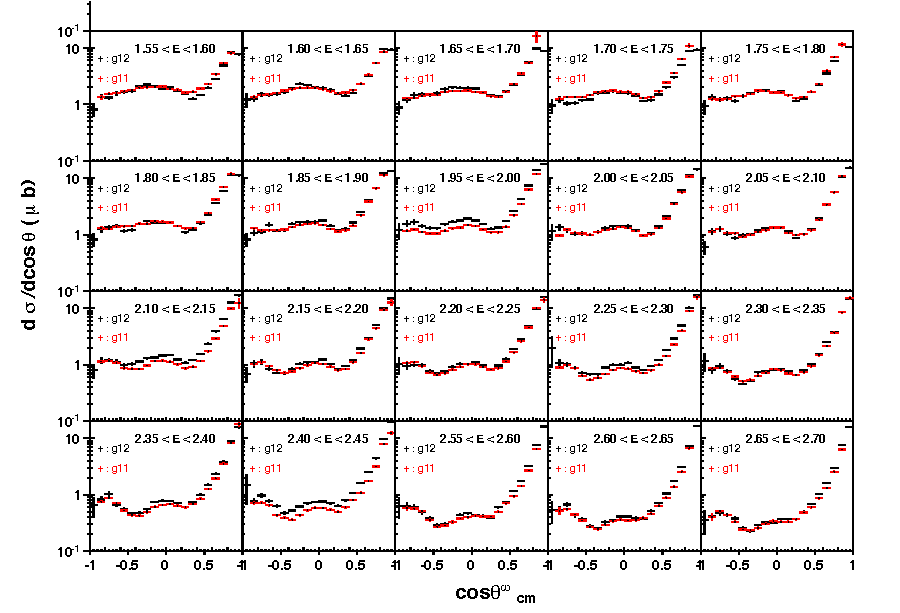
\includegraphics[width=\columnwidth]{{figures/xsec/cross_omega_1}.eps}
\caption[]{\label{fig:xsec.omega1}Differential cross sections for the reaction γ p $\rightarrow$ p ω based on the dominant decay mode ω $\rightarrow$ π$^+$ π$^-$ π$^0$ with a beam energy from 1.5 to 2.5~GeV. Comparison to g11 is in red.}
\end{center}\end{figure}


\begin{figure}[htpb]\begin{center}
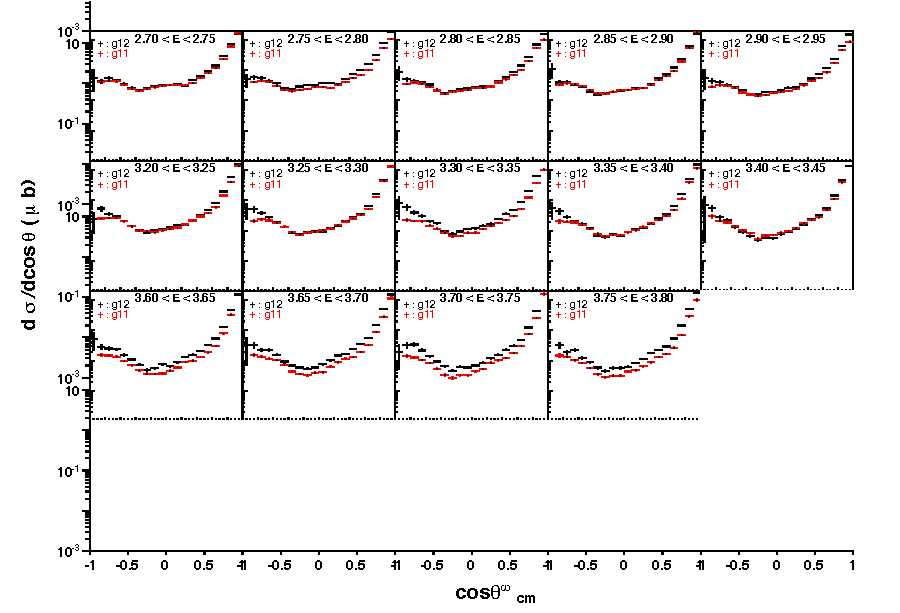
\includegraphics[width=\columnwidth]{{figures/xsec/cross_omega_2}.eps}
\caption[]{\label{fig:xsec.omega2}Differential cross sections for the reaction γ p $\rightarrow$ p ω based on the dominant decay mode ω $\rightarrow$ π$^+$ π$^-$ π$^0$ with a beam energy from 2.5 to 3.65~GeV. Comparison to g11 is in red.}
\end{center}\end{figure}

Furthermore, the $\omega$ yields normalized to the flux as a function of different beam currents has also been studied, in order to verify if there is any trigger/reconstruction inefficiency that is beam current dependent. This is possible since g12 took data at various beam currents at the beginning of the running period.  The variance photon multiplicity, i.e., having more than one photons in the chosen time bucket for the event, has also been taken into account. It can be seen, that the g12 normalized yields for the ω do not have any statistically significant beam current dependency. In fact, the slope in Fig.\ref{fig:xsec.yields} is slightly positive, but still consistent with zero.

In terms of the photon multiplicity, at 60-65nA of the production current, about 87\% of the data has only one photon in the same time bucket chosen for the event, around 12\% has exactly two photons, and approximately 1\% has more than two photons. This issue must addressed by either correcting the cross sections, if one include those events with multiple photons in their analyses, but the photon was chosen randomly. However, one can also address this issue by looping over all photons, and that would not require additional corrections. Since this correction depends on the preference of the individuals, and is rather simple to apply, we do not prescribe/offer a universal procedure per se.


\begin{figure}[htpb]\begin{center}
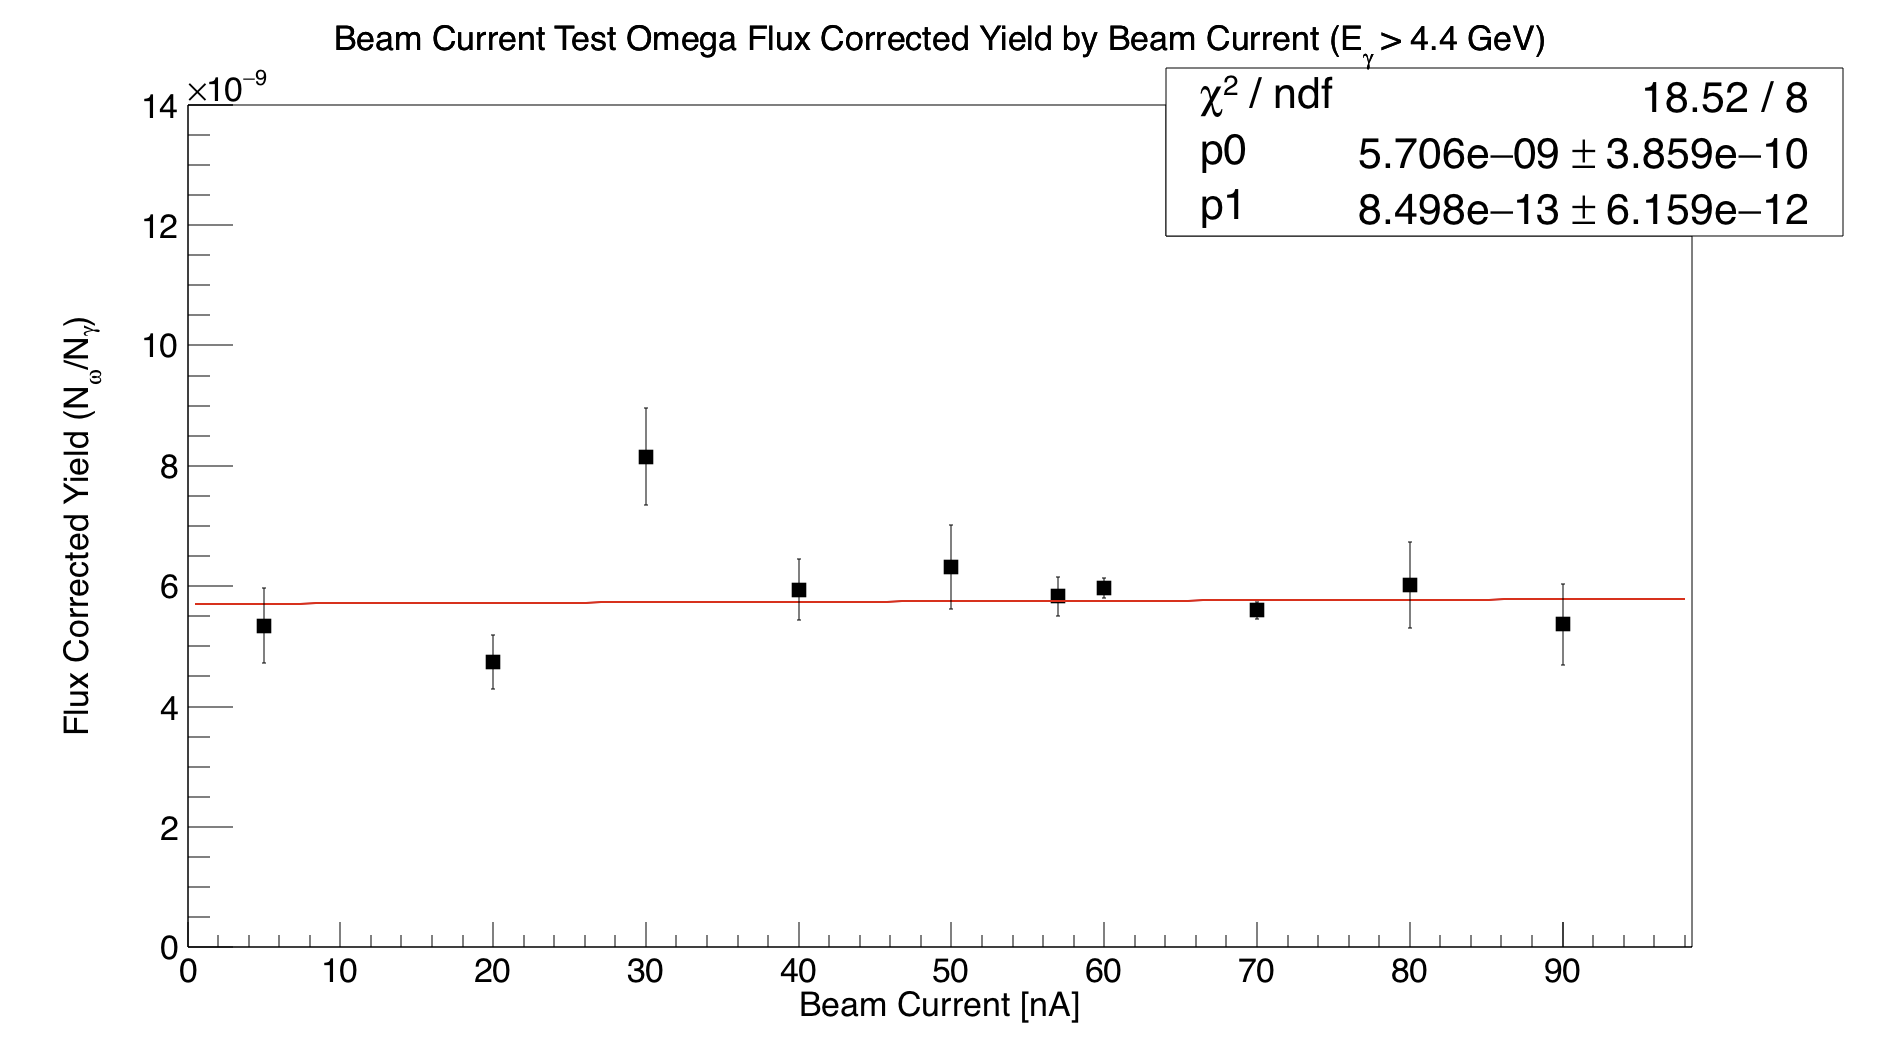
\includegraphics[width=1.1\columnwidth]{{figures/xsec/omegaYieldsCurrent}.png}
\caption[]{\label{fig:xsec.yields}Differential cross sections for the reaction γ p $\rightarrow$ p ω based on the dominant decay mode ω $\rightarrow$ π$^+$ π$^-$ π$^0$ with a beam energy from 2.5 to 3.65~GeV. Comparison to g11 is in red.}
\end{center}\end{figure}

To summarize, the g12 data set does not shown any significant beam-intensity-dependent inefficiency, and the overall normalization, when all corrections documented in this note are applied, can be validated by the consistency between the cross sections such as ω, π$^0$ and Λ when compared with prior results.
